\documentclass[../defence.tex]{subfiles}

\begin{document}
  \begin{frame}{Wafer inhomogeneity - open pore membranes wafer 295}
    \begin{columns}[onlytextwidth, T]
      \column{\dimexpr\linewidth / 21 * 10}
        \begin{block}{Isotherms}
          \scalebox{0.5}{
            \tikzsetnextfilename{295_op}
            \begin{tikzpicture}
                \def\PrelMin{.88}
        				\def\PrelMax{.975}
        				\def\TransMin{1e-7}
        				\def\TransMax{1}
        				\def\LfMin{0}
        				\def\LfMax{2}
                %
                \begin{axis}[
                  /tikz/line join=bevel,
                  grid,
        					axis y line*=left,
                  %legend style={at={(0,0.5)}, legend columns=2, anchor=north west},
                  every axis plot,
        					axis y line*=left,
        					line width = 1pt,
        					xmin = \PrelMin, xmax = \PrelMax,
        					ymin = \LfMin, ymax = \LfMax,
        					xlabel = {Relative pressure $P_\mathrm{rel}$},
        					ylabel = {Liquid fraction $LF$},
        					ytick = {0,0.25,0.50,0.75,1},
                  %title={Open pore membranes of wafer 295},
                  ]
        					% Add plots
        					\addplot[mark=none, color=red] table [x=Prel,y=liquid_fraction]{tikz/graphs/wafer_inhomogeneities/295c_cond_2.txt};
        					%\addlegendentry{$LF_\mathrm{cond}^\mathrm{295c'}$}
        					\addplot[mark=none, color=red!50] table [x=Prel,y=liquid_fraction]{tikz/graphs/wafer_inhomogeneities/295c_evap_2.txt};
        					%\addlegendentry{$LF_\mathrm{evap}^\mathrm{295c'}$}
        					\addplot[mark=none, color=blue] table [x=Prel,y=liquid_fraction]{tikz/graphs/wafer_inhomogeneities/295d_cond_2.txt};
        					%\addlegendentry{$LF_\mathrm{cond}^\mathrm{295d'}$}
                  \addplot[mark=none, color=blue!50] table [x=Prel,y=liquid_fraction]{tikz/graphs/wafer_inhomogeneities/295d_evap_2.txt};
        					%\addlegendentry{$LF_\mathrm{evap}^\mathrm{295d'}$}
        					\addplot[mark=none, color=green] table [x=Prel,y=liquid_fraction]{tikz/graphs/wafer_inhomogeneities/295e_cond_1.txt};
        					%\addlegendentry{$LF_\mathrm{cond}^\mathrm{295e'}$}
        					\addplot[mark=none, color=green!50] table [x=Prel,y=liquid_fraction]{tikz/graphs/wafer_inhomogeneities/295e_evap_1.txt};
        					%\addlegendentry{$LF_\mathrm{evap}^\mathrm{295e'}$}
        					\addplot[mark=none, color=orange] table [x=Prel,y=liquid_fraction]{tikz/graphs/wafer_inhomogeneities/295f_cond_1.txt};
        					%\addlegendentry{$LF_\mathrm{cond}^\mathrm{295f'}$}
        					\addplot[mark=none, color=orange!50] table [x=Prel,y=liquid_fraction]{tikz/graphs/wafer_inhomogeneities/295f_evap_1.txt};
        					%\addlegendentry{$LF_\mathrm{evap}^\mathrm{295f'}$}
        					\addplot[mark=none, color=magenta] table [x=Prel,y=liquid_fraction]{tikz/graphs/wafer_inhomogeneities/295g_cond_1.txt};
        					%\addlegendentry{$LF_\mathrm{cond}^\mathrm{295g'}$}
        					\addplot[mark=none, color=magenta!50] table [x=Prel,y=liquid_fraction]{tikz/graphs/wafer_inhomogeneities/295g_evap_1.txt};
        					%\addlegendentry{$LF_\mathrm{evap}^\mathrm{295g'}$}
                \end{axis}
        				% transmission
        				\begin{axis}[
                  /tikz/line join=bevel,
        					ymode=log,
        					axis y line*=right, ylabel near ticks, yticklabel pos=right,
        					line width = 1pt,
        					xmin = \PrelMin, xmax = \PrelMax,
        					ymin = \TransMin, ymax = \TransMax,
        					ylabel = {Transmission $T$},
        					xtick = {1e-1,1e-2,1e-3},
        					ytick = {10,1,1e-1,1e-2,1e-3},
                  ymajorgrids=true,
                  %legend style={at={(0,0.5)}, legend columns=2, anchor=south west},
        					]
        					% Add plots
        					\addplot[mark=none, color=red] table [x=Prel,y=transmission]{tikz/graphs/wafer_inhomogeneities/295c_cond_2.txt};
        					%\addlegendentry{$T_\mathrm{cond}^\mathrm{295c'}$}
        					\addplot[mark=none, color=red!50] table [x=Prel,y=transmission]{tikz/graphs/wafer_inhomogeneities/295c_evap_2.txt};
        					%\addlegendentry{$T_\mathrm{evap}^\mathrm{295c'}$}
        					\addplot[mark=none, color=blue] table [x=Prel,y=transmission]{tikz/graphs/wafer_inhomogeneities/295d_cond_2.txt};
        					%\addlegendentry{$T_\mathrm{cond}^\mathrm{295d'}$}
                  \addplot[mark=none, color=blue!50] table [x=Prel,y=transmission]{tikz/graphs/wafer_inhomogeneities/295d_evap_2.txt};
        					%\addlegendentry{$T_\mathrm{evap}^\mathrm{295d'}$}
        					\addplot[mark=none, color=green] table [x=Prel,y=transmission]{tikz/graphs/wafer_inhomogeneities/295e_cond_1.txt};
        					%\addlegendentry{$T_\mathrm{cond}^\mathrm{295e'}$}
        					\addplot[mark=none, color=green!50] table [x=Prel,y=transmission]{tikz/graphs/wafer_inhomogeneities/295e_evap_1.txt};
        					%\addlegendentry{$T_\mathrm{evap}^\mathrm{295e'}$}
        					\addplot[mark=none, color=orange] table [x=Prel,y=transmission]{tikz/graphs/wafer_inhomogeneities/295f_cond_1.txt};
        					%\addlegendentry{$T_\mathrm{cond}^\mathrm{295f'}$}
        					\addplot[mark=none, color=orange!50] table [x=Prel,y=transmission]{tikz/graphs/wafer_inhomogeneities/295f_evap_1.txt};
        					%\addlegendentry{$T_\mathrm{evap}^\mathrm{295f'}$}
        					\addplot[mark=none, color=magenta] table [x=Prel,y=transmission]{tikz/graphs/wafer_inhomogeneities/295g_cond_1.txt};
        					%\addlegendentry{$T_\mathrm{cond}^\mathrm{295g'}$}
        					\addplot[mark=none, color=magenta!50] table [x=Prel,y=transmission]{tikz/graphs/wafer_inhomogeneities/295g_evap_1.txt};
        					%\addlegendentry{$T_\mathrm{evap}^\mathrm{295g'}$}
        				\end{axis}
            \end{tikzpicture}}
        \end{block}
        \pause

        \column{\dimexpr\linewidth / 21}
        \column{\dimexpr\linewidth / 21 * 10}
          \begin{block}{Dry transmission measurements}
            \scalebox{0.45}{
              \tikzsetnextfilename{wafer_295_transmission}
              %\tikzexternaldisable
              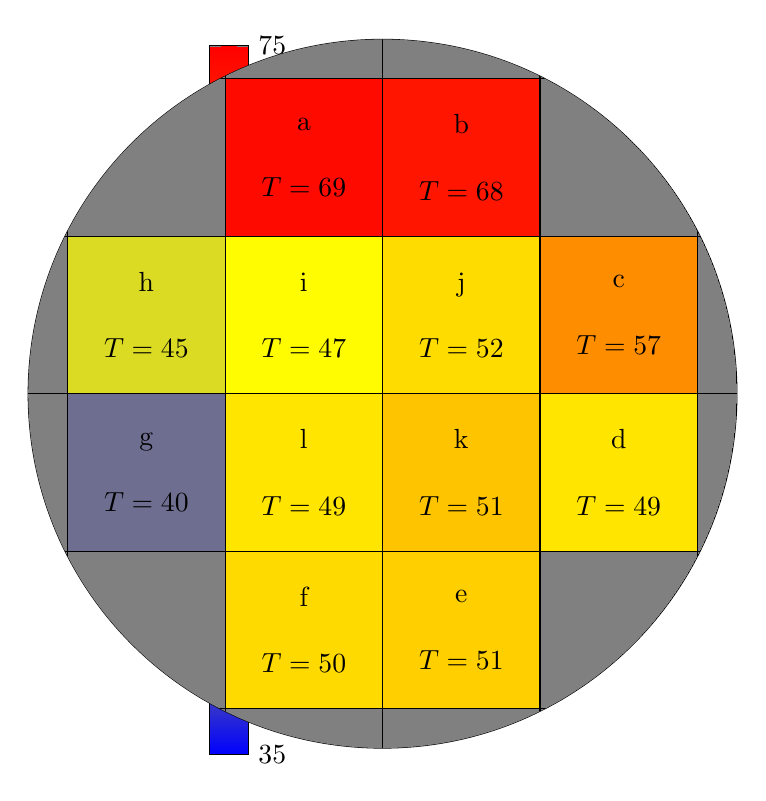
\begin{tikzpicture}
                \begin{scope}[xshift=-2.5cm,yshift=-3cm]
                  \begin{axis}[
                      hide axis,
                      colormap/hot,
                      xmin=-4.5, xmax=4.5,
                      ymin=-4.5, ymax=4.5,
                      height=9cm,
                      width=9cm,
                      axis equal,
                      colorbar,
                      point meta min=35,
                      point meta max=75,
                      colorbar style={
                        width=0.5cm,
                        height=9cm,
                        xtick={35,40,...,70}
                      }
                  ]
                  \end{axis}
                \end{scope}
                      \clip[draw] (0,-0) circle (4.5);
                      \fill[gray] (0,-0) circle (4.5);
                      \fill[/utils/exec={\pgfplotscolormapdefinemappedcolor{500}}, color of colormap=971] (-2,4) -- (0,4) -- (0,2) -- (-2,2) -- cycle;
                      \node[align = center] at (-1,3) {a\\ \\ $T = \SI{69}{\percent}$};
                      %b
                      \fill[/utils/exec={\pgfplotscolormapdefinemappedcolor{500}}, color of colormap=942] (0,4) -- (2,4) -- (2,2) -- (-0,2) -- cycle;
                      \node[align = center] at (1,3) {b\\ \\ $T = \SI{68}{\percent}$};
                      %c
                      \fill[/utils/exec={\pgfplotscolormapdefinemappedcolor{500}}, color of colormap=629] (2,2) -- (2,0) -- (4,0) -- (4,2) -- cycle;
                      \node[align = center] at (3,1) {c\\ \\ $T = \SI{57}{\percent}$};
                      %d
                      \fill[/utils/exec={\pgfplotscolormapdefinemappedcolor{500}}, color of colormap=400] (2,0) -- (4,0) -- (4,-2) -- (2,-2) -- cycle;
                      \node[align = center] at (3,-1) {d\\ \\ $T = \SI{49}{\percent}$};
                      %e
                      \fill[/utils/exec={\pgfplotscolormapdefinemappedcolor{500}}, color of colormap=457] (0,-2) -- (2,-2) -- (2,-4) -- (0,-4) -- cycle;
                      \node[align = center] at (1,-3) {e\\ \\ $T = \SI{51}{\percent}$};
                      %f
                      \fill[/utils/exec={\pgfplotscolormapdefinemappedcolor{500}}, color of colormap=429] (-2,-2) -- (0,-2) -- (0,-4) -- (-2,-4) -- cycle;
                      \node[align = center] at (-1,-3) {f\\ \\ $T = \SI{50}{\percent}$};
                      %g
                      \fill[/utils/exec={\pgfplotscolormapdefinemappedcolor{500}}, color of colormap=143] (-4,0) -- (-2,0) -- (-2,-2) -- (-4,-2) -- cycle;
                      \node[align = center] at (-3,-1) {g\\ \\ $T = \SI{40}{\percent}$};
                      %h
                      \fill[/utils/exec={\pgfplotscolormapdefinemappedcolor{500}}, color of colormap=286] (-4,2) -- (-2,2) -- (-2,0) -- (-4,0) -- cycle;
                      \node[align = center] at (-3,1) {h\\ \\ $T = \SI{45}{\percent}$};
                      %i
                      \fill[/utils/exec={\pgfplotscolormapdefinemappedcolor{500}}, color of colormap=343] (-2,2) -- (0,2) -- (0,0) -- (-2,0) -- cycle;
                      \node[align = center] at (-1,1) {i\\ \\ $T = \SI{47}{\percent}$};
                      %j
                      \fill[/utils/exec={\pgfplotscolormapdefinemappedcolor{500}}, color of colormap=425] (0,2) -- (2,2) -- (2,0) -- (0,0) -- cycle;
                      \node[align = center] at (1,1) {j\\ \\ $T = \SI{52}{\percent}$};
                      %k
                      \fill[/utils/exec={\pgfplotscolormapdefinemappedcolor{500}}, color of colormap=486] (0,0) -- (2,0) -- (2,-2) -- (0,-2) -- cycle;
                      \node[align = center] at (1,-1) {k\\ \\ $T = \SI{51}{\percent}$};
                      %l
                      \fill[/utils/exec={\pgfplotscolormapdefinemappedcolor{500}}, color of colormap=400] (-2,0) -- (0,0) -- (0,-2) -- (-2,-2) -- cycle;
                      \node[align = center] at (-1,-1) {l\\ \\ $T = \SI{49}{\percent}$};
                      \draw[step=2] (-4.5,-4.5) grid (4.5,4.5);
              \end{tikzpicture}}
          \end{block}
    \end{columns}
  \end{frame}
\end{document}
